\documentclass[12pt, a4paper, onecolumn]{article}


%package pour rétrécir les marges
\usepackage[margin=64pt]{geometry}

%package pour les équations mathématiques
\usepackage{amsmath}

%package pour les tableaux (pour l'annexe 1)
\usepackage{array}

%package et commande pour les alinéas
\usepackage{tabto}
\renewcommand{\tab}{\tabto{15px}}

%pacakges pour la bibliographie
\usepackage[toc,page]{appendix}
\usepackage{hyperref}
\usepackage[super]{natbib}

%package pour le signe € 
\usepackage{eurosym}

%package pour les couleurs (utiles pour les références)
\usepackage{xcolor}

%packages pour les graphes (conversions eps -> pdf et affichage)
\usepackage{graphicx}
\usepackage{epstopdf}
\usepackage{subfigure}
\usepackage{float}

%packages pour rajouter des sous-sous-titres
\usepackage{titlesec}
\usepackage{scrextend}
\usepackage{changepage}
\setcounter{secnumdepth}{3}

%commande permettant de citer plusieurs sources à la fois (le package permet la création de la fonction récursive)
\usepackage{etoolbox}
\makeatletter
\newcommand{\csvdel}{}
\newcommand{\bettercite}[1][,]{%déclaration de la fonction générale
  \renewcommand{\csvdel}{\renewcommand{\csvdel}{}}%lors de l'appel commence par rajouter un crochet
  \csname\endcsname$^[$\checknextarg}
\newcommand{\checknextarg}{\@ifnextchar\bgroup{\gobblenext}{}}%vérifie si un autre argument existe
\newcommand{\gobblenext}[1]{\csvdel\textcolor{blue}{\textbf{\cite{#1}}}\@ifnextchar\bgroup{$^,$\gobblenext}{$^]$}}%récupère l'argument qui suit, met la source et une , s'il existe sinon ferme le crochet
\makeatother

%commande pour mieux citer les annexes et figures/images
\newcommand{\cfannexe}[1]{\textsuperscript{(\textcolor{blue}{\textbf{\ref{annexe #1}}})}}
\newcommand{\cffig}[1]{\textsuperscript{\{\textcolor{blue}{fig.\textbf{\ref{#1}}}\}}}

%packages et commandes pour surligner le numéro de la figure
\usepackage{ulem}
\usepackage{caption}[2007/09/01] % needs v3.1 or newer
\DeclareCaptionLabelFormat{underlcap}{\uline{#1 #2}}
\captionsetup[figure]{labelformat=underlcap} 

%Evite l'apparition de traits d'unions pour séparer les mots sur plusieurs lignes
\tolerance=1
\emergencystretch=\maxdimen
\hyphenpenalty=10000
\hbadness=10000



%définition du titre des auteurs et autres informations clé
\title{Comparaison des performances entre les technologies maglev et ferroviaires actuelles}
\author{Mathieu Denglos, Kerian Chauvin}
\date{}



\begin{document}


%page 1
\maketitle  %titre

\begin{figure}[H] %image d'introduction
  \centering
  \scalebox{0.28}
  {\includegraphics{img/image_couverture.png}}
\end{figure}



\pagebreak %page 2
\section*{Abstract} %Résumé
\tab Avec les enjeux écologiques devenus prépondérants lors des dernières années, les différents gouvernements se tournent de plus en plus vers le transport ferroviaire car plus écologique.
Cependant, les trains ne sont pas les seuls véhicules guidés ayant un fort potentiel en terme écologique, ainsi qu’en terme de performances.
Les médias parlent assez régulièrement des technologies maglev comme des véhicules très rapides et ayant un fort potentiel.\\
\tab Pour comparer ce fort potentiel, il est primordial de prendre en compte tous les aspects techniques qui caractérisent les performances du système.
Or, les études déjà menées sur les véhicules maglev ne comparent que rarement ces deux systèmes, et généralement que sur des points spécifiques. \\
\linebreak
\tab C’est pour cela que nous avons décidé, dans une même étude, de regrouper une comparaison objective de ces différentes caractéristiques techniques, afin de déterminer les potentiels bénéfices des technologies maglev sur celles des trains, et dans quels cas il est judicieux de s’orienter vers une technologie ou une autre. \\
\linebreak
\tab Contrairement à ce que le grand public peut penser des technologies maglev, les capacités techniques évoquées dans les médias ne sont pas généralisées à tous les maglev.
La combinaison de nos résultats nous permet aussi de conclure qu’aucune technologie ne ressort et que selon le trajet ou les contraintes techniques, une étude au cas par cas est nécessaire pour déterminer quelle technologie serait la plus adéquate. \\

\section*{Introduction} %Introduction
\tab Les véhicules maglev sont souvent montrés par les médias et présents dans l’imaginaire collectif comme étant le transport guidé de l’avenir, aux vitesses phénoménales.
En vérité, une telle conclusion n’est pas directement envisageable.
Ces technologies sont bien plus complexes et subtiles qu’on puisse le penser.
Pour un spectateur extérieur, les véhicules maglev et les trains sont très similaires.
Leurs structures sont similaires, la seule différence notable provenant du contact roue-rail, manquant sur les maglev et remplacé par des technologies de lévitation. \\
\linebreak
\tab Ces différents aspects nous amènent à nous demander ce qui peut différencier les technologies maglev avec celles des trains, principalement sur leurs performances, tout en se questionnant sur l’influence du contact roue-rail. \\
\tab Avant de comparer ces différentes technologies, nous ferons une description des technologies étudiées, importante pour l’explication des résultats sur les performances du système. \\
\linebreak
\tab Il est important de mentionner que tout au long de cette étude des projets tels que l’hyperloop ne seront pas cités car, ceux-ci voyageant à pression réduite, la traînée aérodynamique diminue fortement (jusqu'à 10 fois)\bettercite{maglevintube}, faussant les potentiels résultats recueillis.
De plus, nous ne nous intéresserons qu’aux automotrices électriques alimentées par caténaire dans le cas des trains, pour se rapprocher le plus possible des véhicules maglev. \\



\pagebreak %page 3
\section{Présentation des technologies étudiées} %Partie 1 : technologies étudiées
\tab Contrairement aux systèmes relativement normalisés du ferroviaire moderne, les systèmes maglev sont multiples et chacun possède ses avantages et ses inconvénients.
En raison du nombre d'études et de lignes ouvertes, deux technologies de propulsion retiennent notre attention :
\begin{itemize}
  \item la propulsion LIM à stator court (Linear Induction Motor),
  \item la propulsion LSM à stator long (Linear Synchronous Motor).
\end{itemize}
\tab Avant de répondre à notre problématique il est important de détailler le fonctionnement de ces différentes technologies peu connues.

\subsection{Technologies des trains}
\tab Le fonctionnement des trains se base sur une technologie vieille de 5 siècles, le guidage d’un véhicule à roues par l’utilisation de rails. \\
\tab La traction ferroviaire électrique par caténaire est permise tout d'abord par une alimentation continue ou monophasée.
Après diverses transformations à l'aide de hacheurs, de redresseurs ou d'onduleurs, celle-ci alimente les moteurs du train. \\
\linebreak
\tab On distingue trois types de moteurs électriques utilisés dans le ferroviaire : le moteur à courant continu, le moteur synchrone et le moteur asynchrone. \\
\tab Le moteur à courant continu reçoit une alimentation continue.
Le stator, en étant alimenté, va créer un champ magnétique en son sein et ainsi permet d'entraîner en rotation le rotor qui s'y trouve. \\
\tab Le stator des moteurs synchrone et asynchrone reçoit quant à lui une alimentation triphasée, les trois phases alimentant ainsi les trois bobines du stator, créant un champ tournant.
Dans le cas d'un moteur synchrone, le rotor, constitué d'un aimant permanent ou bien d'une bobine alimentée en courant continu, va suivre ce champ et donc être entraîné en rotation.
Dans le cas d'un moteur asynchrone, le rotor est constitué de spires fermées et indépendantes qui vont être le siège de courants induits quand le rotor est soumis au champ tournant.
Elles vont ainsi l'entraîner en rotation en essayant de ratrapper ce champ. \\
\tab Ces moteurs permettent par la suite d'entraîner en rotation les essieux moteurs du train et donc de le mettre en mouvement.
Ceci est permis par l’adhérence, bien que faible, entre la roue et le rail, principale différence entre le train et les véhicules maglev.

%Images train
\begin{figure}[H]
  \centering
  \begin{minipage}{0.5\textwidth}
    \includegraphics[width=\textwidth]
    {img/adherence.jpg}
    \caption{représentation du contact roue-rail}
    \label{adherence}
  \end{minipage}\hfill
  \begin{minipage}{0.5\textwidth}
    \includegraphics[width=\textwidth]
    {img/bogietrain.png}
    \caption{bogie de tgv}
    \label{bogietrain}
  \end{minipage}
\end{figure}



\pagebreak %page 4
\subsection{Technologies LIM et EMS}
\tab La technologie maglev à moteur à induction linéaire (LIM) est la première des deux technologies actuellement déployées.
Comme tout moteur, le LIM est constitué de deux parties : le rotor, se situant sous le véhicule et étant la partie alimentée du moteur, et le stator composé d'une plaque en acier sur de l'aluminium, se situant sur le rail.
Le rotor, situé sur le train est alimenté et va générer un champ magnétique parallèle au rotor.
Ce champ magnetique va induire un courant dans le rail (d'après la loi de Lenz) qui lui-même va générer un champ magnétique parallèle au stator (donc au rotor) et de sens opposé à celui du rotor.
Ces deux champs magnétiques s’opposent, repoussant le rotor et faisant avancer le train\bettercite{coloradomaglev}\cffig{schemaLIM}. \\
\linebreak
\tab La motorisation n'est pas le seul aspect technique à étudier afin de répondre à notre problématique.
La technologie de sustentation est tout aussi impactante sur les performances du véhicule.
Dans le cas des maglevs à LIM, c'est la sustentation electromagnétique (EMS) qui est le plus communément utilisée.
La technologie EMS est constituée de deux séries d'électro-aimants attachées au véhicule et situées sous le rail pour la sustentation, ainsi que sur les côtés pour le guidage\cffig{schemaEMS}.
Quand ceux-ci sont alimentés, ils sont attirés par le rail, lévitant le train par dessous pour les aimants de sustentation et permettant la stabilité du véhicule pour les aimants de guidage \bettercite{maglevtech}.
Des capteurs sont situés autour des aimants de sustentation, permettant, en régulant la puissance envoyée dans les électro-aimants, de garder une distance entre le LIM et le rail constant (généralement de 8 $\pm$ 3mm\bettercite{koreamaglevprogram}). \\

\begin{figure}[H]
  \centering
  \begin{minipage}{0.45\textwidth}
    \includegraphics[width=\textwidth]
    {img/schemaLIM.png}
    \caption{schéma fonctionnement LIM}
    \label{schemaLIM}
  \end{minipage}\hfill
  \begin{minipage}{0.45\textwidth}
    \includegraphics[width=\textwidth]
    {img/schemaEMS.png}
    \caption{schéma fonctionnement EMS}
    \label{schemaEMS}
  \end{minipage}\par
  \vskip\floatsep% normal separation between figures
  \includegraphics[width=0.68\textwidth]
  {img/bogieLIM.png}
  \caption{bogie du Changsha maglev express\bettercite{changshasources}}
  \label{bogieLIM}
\end{figure}



\pagebreak %page 5
\subsection{Technologies LSM et EDS}
\tab L’autre technologie développée est la technologie maglev à moteur lineaire synchrone (LSM).
Comme pour le LIM, le LSM est divisé en deux parties, le rotor et le stator.
Cependant, son fonctionnement diffère totalement de celui du LIM.
Le rotor (situé sur le train) est composé d’aimants permanents avec une polarité alternée (N,S,N,...). Le stator (situé sur le rail) est composé d’électro-aimants ayant eux aussi des polarités alternées.
Cette technologie utilise le principe fondamental des aimants qui s’attirent lorsque leurs polarités s’opposent.
Lorsque les électroaimants du rail sont alimentés, ils se comportent comme des aimants, et donc ils attirent les pôles des aimants du train.
Cependant, dès que les pôles sont opposés, le train devrait s’arrêter, on change alors le sens du courant dans les bobines, pour inverser les pôles des électroaimants.
Le pôle Sud du train est alors attiré par un nouveau pôle Nord un peu plus loin sur le rail, et ainsi tout le long du trajet\bettercite{coloradomaglev}\cffig{schemaLSM}. \\
\linebreak
\tab Pour la sustentation, les systèmes LSM sont associés avec une sustentation électrodynamique (EDS).
Celle-ci, contrairement au système EMS, utilise le principe de répulsion des aimants de même polarité.
La voie inclut, en plus des bobines pour le moteur linéaire, des bobines pour faire léviter le train.
Ce système ce situe généralement sous le train, ou sur les côtés\cffig{schemaEDS} tel que sur la ligne Chuo Shinkansen.
Malheureusement, ce système ne suffit pas étant donné qu'il ne fonctionne que sur des moyennes et fortes vitesses (supérieures à 100km/h).
Pour subvenir aux besoins pour les petites vitesses, la technolgie EDS est combinée avec un système EMS ou des roues\bettercite{maglevtech}.
Pour finir, certaines lignes combinent la sustentation avec de la supraconductivité (amenant le système à des températures très faibles) pour améliorer les performances.

\begin{figure}[H]
  \centering
  \begin{minipage}{.51\linewidth}
    \includegraphics[width=\textwidth]{img/schemaLSM.png}
    \caption{schéma fonctionnement LSM}
    \label{schemaLSM}
  \end{minipage}
  \begin{minipage}{.48\linewidth}
    \includegraphics[width=\textwidth]{img/voirie.png}
    \caption{éléments de voirie}
    \label{schemaEDS}
    \includegraphics[width=\textwidth]{img/bogieLSM.jpg}
    \caption{bogie MLX-01 (Chuo Shinkansen)}
    \label{bogieLSM}
  \end{minipage}
\end{figure}



\pagebreak %page 6
\subsection*{Comparaison fonctionnelle de ces technologies}

\tab Bien que ces deux technologies maglev seront étudiées sur les mêmes points afin de répondre à notre problématique générale, il reste important de déterminer laquelle se rapproche le plus du train, ce qui nous permettra de nous intéresser à notre problématique secondaire sur l'impact du contact roue-rail sur les performances.
Le meilleur moyen pour trouver la technologie maglev se rapprochant plus du train sans rentrer tout de suite dans des données techniques est de comparer leurs chaînes de traction. \\

\begin{figure}[H]
  \centering
  \begin{minipage}[H]{0.47\textwidth}
    \includegraphics[width=\textwidth]{img/CTCtrain.png}
    \;(a) train à moteur continu
  \end{minipage}
  \hfill
  \begin{minipage}[H]{0.47\textwidth}
    \includegraphics[width=\textwidth]{img/CTCLIM.png}
    \;(b) maglev LIM
  \end{minipage}\par
  \vskip\floatsep\par
  \vskip\floatsep

  \begin{minipage}[H]{0.47\textwidth}
    \includegraphics[width=\textwidth]{img/CTAtrain.png}
    \;(c) train à moteur synchrone/asynchrone
  \end{minipage}
  \hfill
  \begin{minipage}[H]{0.47\textwidth}
    \includegraphics[width=\textwidth]{img/CTALSM.png}
    \;(d) maglev LSM
  \end{minipage}
  \caption{Chaines de tractions}
\end{figure}

\tab On constate en comparant les chaînes de traction ci-dessus que celle de la technologie de propulsion LIM se rapproche le plus de celle du train à moteurs continus.
Ceci est logique car le fonctionnement global reste similaire comparé à nos trains actuels, la seule différence notable venant du contact roue-rail qui engendre la nécessité de convertir le moteur rotationnel en moteur linéaire. \\
\linebreak
\tab La chaîne de traction de la propulsion LSM diffère totalement de celle des trains actuels.
Dans ce cas la différence trouvée est aussi logique car les technologies LSM ne nécessitent aucun système d'alimentation interne au train, à part pour les éléments auxiliaires (lumière, chauffage…).
En effet, la majeure partie de la propulsion se situe sur le rail lui-même.
Nous avons tout de même apporté un intérêt fort à cette technologie car c’est elle qui nous permettra de remettre en question la vision généralisée des systèmes maglev avec les résultats que nous avons trouvés.\\



\pagebreak %page 7
\section{Critères de choix}

\tab Notre objectif étant de comparer les deux technologies maglev à celles des trains, nous allons donc les comparer sur trois axes principaux :
\begin{itemize}
  \item Le trajet : comparaison des différents paramètres influant sur les temps de trajets,
  \item Le coût : destination des investissements aux différents instants de la vie d’une ligne,
  \item Autres critères pouvant influencer le choix du type de réseau.
\end{itemize}

\subsection{Trajet}
\tab Lors de l’analyse d’un système de transport, la caractéristique la plus importante du point de vue utilisateur est le temps de trajet.
Celui-ci est principalement influencé par la vitesse du train, mais aussi ses capacités d’accélération et de décélération.

\begin{addmargin}[30px]{0px} \subsubsection*{Vitesse}\end{addmargin}
\tab Commençons par rappeler les vitesses commerciales maximales des trains roulant sur les différents réseaux ferroviaires de nos jours. Celles-ci sont généralement limitées entre 320 km/h et 360 km/h pour les lignes à grande vitesse. \\
\tab Dans les médias, les véhicules maglev sont toujours représentés comme des technologies bien plus rapides ; cependant, il faut faire la distinction entre les deux technologies car les résultats varient énormément. \\
\linebreak
\tab En commençant par nous intéresser à la technologie de propulsion LIM, nous trouvons des résultats bien inférieurs à ceux énoncés pour les trains et en opposition avec la vision du grand public.
En effet, les vitesses commerciales maximales sur les lignes ouvertes ne dépassent jamais les 120km/h\cfannexe{1}.
Des recherches plus approfondies ont montré que même si cette technologie était optimisée, les vitesses resteraient aux alentours des 160 km/h\bettercite{optimisationchangsha}. \\
\linebreak
\tab C’est en recherchant dans les technologies LSM que les résultats semblent bien plus intéressants.
En effet, les vitesses atteintes avec ce matériel roulant dépassent les 400 km/h pour des technologies de sustentations EDS classiques et peuvent être poussées jusqu'à 550-600 km/h pour de l’EDS couplé à de la supraconductivité\cfannexe{1}. \\
\linebreak
\tab Bien que pour tout type de transport, la vitesse est un point important, dans le cadre d’un système guidé, la sécurité reste primordiale et est le premier point pris en considération lors de l’implémentation de systèmes.
La vitesse est un point important à surveiller car le risque d’instabilité et donc de déraillement augmente fortement avec la vitesse.
Pour justifier les résultats précédemment cités, il est important de s'intéresser aux vitesses où l’instabilité devient trop importante, aussi appelée vitesse critique.
Ces vitesses critiques peuvent être influencées par différents facteurs contrôlables ou non par le constructeur.
Pour l'augmenter, le constructeur peut par exemple diminuer la masse du bogie ou améliorer les dispositifs de stabilisation de celui-ci.
Il est donc important de comprendre que ces résultats sont impactés par le matériel roulant choisi et que les résultats exprimés ci-dessus ne peuvent prendre en compte toutes les situations. Cependant dans le cas de notre étude, ces ordres restent suffisants pour émettre une conclusion quant à l'impact des différentes technologies sur la vitesse critique. \\
\linebreak
\tab Pour les trains actuellement en service, selon les pays et les conditions cités ci-dessus, la valeur relevée varie entre 430 km/h (pour les sols plus meubles) et 580 km/h (pour les sols plus durs)\bettercite{vitessecritiquetrain}.
Sachant qu'en plus des points cités précédemment, les constructeurs ferroviaires jouent sur d'autres paramètres pour améliorer la stabilité du bogie tel que l'empattement (pouvant atteindre 3 mètres pour les TGV) et la conicité des roues. \\
\linebreak
\tab Pour les technologies LIM, la vitesse critique est faible, elle tourne aux alentours de 250 km/h\bettercite{vitessecritiquelim} pour un écart entre le moteur et le rail de 8mm (distance la plus communément retrouvée) et est proportionnelle à cet écart. \\
\tab Celle-ci n’est pas directement induite par la technologie de propulsion, mais principalement par la technologie de sustentation.
En effet les technologies de sustentation EMS nécessitent un espacement très précis (à quelques millimètres près), espacement qui peut être difficilement gardé à forte vitesse et qui augmente les risques d’accidents. \\
\linebreak
\tab Pour les technologies LSM, la vitesse critique est compliquée à calculer car celle-ci dépend de beaucoup de variables qui peuvent drastiquement changer le résultat.
Cependant pour donner une fourchette large en prenant en compte les conditions d’utilisation, la vitesse critique pour les systèmes LSM est entre 700 km/h et 900km/h\bettercite{vitessecritiquelsm}. \\
\tab Contrairement à la sustentation EMS qui devient rapidement instable, les technologies de sustentations EDS qui sont liées à la propulsion LSM restent stable même à très grandes vitesses, de plus, l’utilisation de supraconductivité améliore encore plus la stabilité globale, et permet donc des vitesses plus élevées.\\
\linebreak
\tab Avec ces informations, nous pouvons déjà conclure quant aux potentiels programmes de traction que chaque technologie peut réaliser.
En effet, les programmes de traction des trains à grandes vitesses et des technologies maglev LSM peuvent parfaitement subvenir aux besoins pour de longues distances grâce à leurs fortes vitesses, alors que les technologies LIM qui ont des capacités de vitesses limitées pourront convenir à des réseaux de plus courtes distances, tel que des métros, VAL ou des Réseaux Express Régionaux.
Bien que le programme de traction dépend de plus de facteurs, nos hypothèses se confirment lorsque nous regardons les trajets empruntés par les lignes déjà existantes\cfannexe{1}. \\

\begin{addmargin}[30px]{0px} \subsubsection*{Accélération et décélération}\end{addmargin}
\tab Bien que la vitesse soit un point primordial pour le temps de voyage, celle-ci n’est pas le seul point influençant celui-ci.
La capacité d’accélération et de décélération peuvent aussi grandement améliorer ce point là. \\
\linebreak
\tab La capacité d’accélération et de décélération du train est un de ses grands défauts, causé principalement par la faible adhérence du contact roue-rail.
D’après les chiffres de SNCF réseau, la décélération minimale imposée pour les trains de voyageurs est de 0.5m/s² pour une vitesse inférieure à 160km/h et 0.6 m/s² pour une vitesse supérieure à 160 km/h\bettercite{decelerationtrain}.
Pour les LIM, l’accélération est entre 0.9 et 1.1 m/s² et la décélération est de 1.1 m/s² et atteint les 1.3m/s² en cas de freinage d’urgence\bettercite{changshadata}{incheonairport}{linimo}.
Pour les LSM, la décélération et l’accélération se situe à 1.6m/s² et atteint jusqu’à 2,4m/s² en cas de freinage d’urgence\bettercite{maglevus}.\\
\tab Comme pour tout système, l’accélération des véhicules guidés peut être exprimée grâce au PFD.
Pour les véhicules guidées, le PFD s’écrit simplement : \\
$$kM\gamma = R_{traction} - R_{r\acute{e}sistant}$$   %page 8
\tab Il y a donc trois facteurs pouvant augmenter la valeur de l’accélération : \\

\begin{itemize}
  \item l'augmentation de l'effort de traction,
  \item la diminution de l'effort résistant,
  \item la diminution de la masse.
\end{itemize}
\tab L’augmentation de l’effort de traction ne sera pas étudiée ici car celui-ci varie drastiquement selon le programme de traction associé\cfannexe{2}.
Il est cependant possible de l’augmenter en ajoutant de la motorisation ou en améliorant la puissance de celle-ci.
Cependant cette décision a un fort impact sur la masse transportée et sur le coût. \\
\linebreak
\tab L'effort résistant est généré par la résistance à l'avancement des véhicules ainsi que par le profil de la voie. On a alors :
$$R_{r\acute{e}sistant} = R_{av} + R_p$$
La résistance R$_p$ dépendant uniquement du profil de voie (déclivité et/ou courbure) et non directement de la technologie de propulsion, celle-ci sera considérée nulle dans cette partie.
Quant à la résistance à l'avancement, on a une équation quadratique dépendant de la vitesse et de la forme :
$$R_{av} = A + BV + CV^2$$
\tab A grande vitesse (entre 320 et 360 km/h), plage qui nous intéresse, les termes A et BV sont négligeables.
Selon les mesures effectuées sur différents trains et véhicules maglev, les valeurs de résistance à l’avancement trouvées sont dans le même ordre de grandeur\bettercite{ei}, montrant une certaine constance du coefficient C. \\
\tab En effet, le coefficient aérodynamique C caractérise la pénétration de l'air par le véhicule.
Il est donc indépendant de la technologie de propulsion.
Le coefficient A dépend de la résistance mécanique, notamment de la masse des caisses, tandis que le coefficient B dépend bien plus de la technologie de propulsion et correspond aux autres paramètres du véhicule, notamment sa puissance, le contact roue-rail dans le cas des trains ou bien la résistance générée par le moteur dans le cas des maglev.
Le coefficient B est ainsi celui qui diffère le plus entre les technologies\bettercite{thesetgv}{ei}. \\
\tab La traînée dynamique causée par le contact roue-rail des trains ne représente que 10\% de la résistance à l'avancement\bettercite{maglevintube}, d'où la faible différence des efforts résistifs. \\
\linebreak
\tab La diminution de la masse est le point le plus flagrant.
Afin de comparer la masse des véhicules selon leurs modes de propulsion, nous utilisons ici la masse surfacique (en kg/m²) ainsi que la longueur des véhicules.
En effectuant le calcul $\sigma = \frac{m}{S}$ pour chacun des 3 modes de propulsion étudiés, et en prenant la valeur moyenne sur les différentes lignes étudiées, nous trouvons les résultats suivants pour les technologies à dessertes régionales :
\begin{itemize}
  \item $\sigma_{train} = 660kg/m^2$
  \item $\sigma_{LIM} = 530kg/m^2$\bettercite{koreamaglevprogram}{changshadata}{linimo}
\end{itemize}
Et pour les grandes lignes :
\begin{itemize}
  \item $\sigma_{train} = 830kg/m^2$\bettercite{thesetgv}
  \item $\sigma_{LSM} = 650kg/m^2$\bettercite{ei}
\end{itemize}

\tab Ces résultats ne sont pas étonnants aux vues des technologies mises en jeu.
Les technologies de propulsion des trains régionaux et LIM étant relativement proches, leur masse surfacique le sont logiquement aussi.
Les véhicules LSM ressortent des trains par leur masse surfacique plus faible en raison de l’absence de technologies de propulsion dans le train même, celles-ci étant concentrées sur la voie.
De plus, les véhicules maglev restent plus courts que les trains.
Avec 30m à 50m de long pour les véhicules LIM et 80m à 120m de long pour les véhicules LSM contre 200m (en unité simple) à 450m (en unité multiple) de long pour le train. \\
\linebreak
\tab Dans l’ensemble, ces différents points sont en faveur des technologies maglev, qui restent bien plus efficaces sur leur accélération et décélération en comparaison aux trains. \\
\tab Cependant pour nous rapporter au temps de trajet, nous allons nous ramener au temps de trajet.
C’est dans cette optique que nous allons nous intéresser au temps perdu par ces différentes technologies lors d’un arrêt en gare.
Nous considérerons ici uniquement les valeurs commerciales et non les valeurs de freinage d’urgence, ainsi qu'un temps d'arrêt nul.
Afin de calculer le temps perdu, nous utilisons la formule : \\
$$t_{perdu}(V) = t_{d\acute{e}c\acute{e}l\acute{e}ration}(V) + t_{acc\acute{e}l\acute{e}ration}(V) \; – \; \frac{d_{parcourue}(V)}{V}$$
\noindent Avec :
\begin{itemize}
  \item $t_{perdu}(V)$ : le temps que le véhicule perd pour s’arrêter à partir d’une vitesse V et revenir à cette vitesse (exemple : lors d'un arrêt en gare),
  \item $t_{d\acute{e}c\acute{e}l\acute{e}ration}(V)$ : le temps que met le véhicule pour passer de la vitesse V à 0 km/h,
  \item $t_{acc\acute{e}l\acute{e}ration}(V)$ : le temps que met le véhicule pour passer de 0 km/h à la vitesse,
  \item $d_{parcourue}(V)$ : la distance théorique qu'aurait parcouru à vitesse constante le véhicule pendant la durée de la phase de décélération/accélération.
\end{itemize}

\begin{figure}[H]
  \centering
  \scalebox{0.48}
  {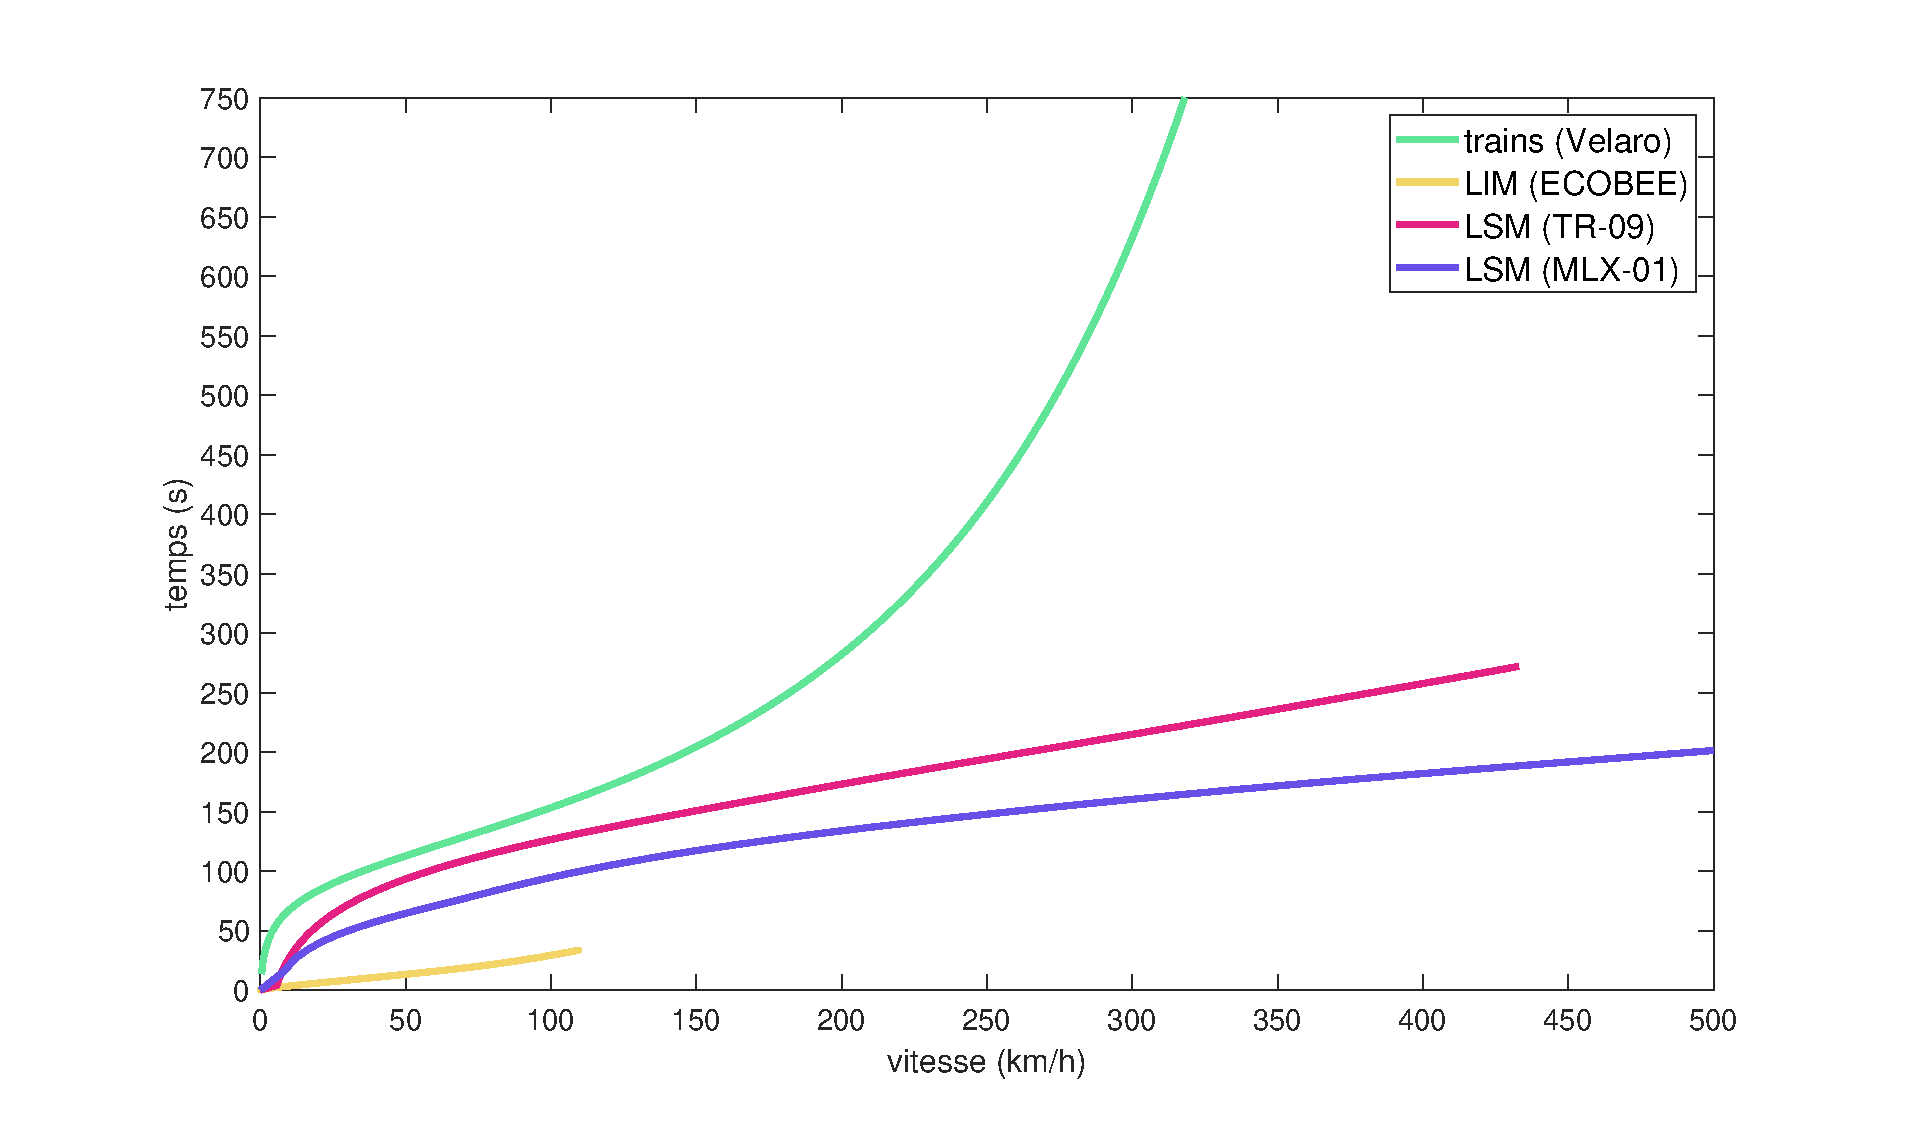
\includegraphics{fig/TP.eps}}
  \label{temps perdu}
  \caption{temps perdu par arrêt en fonction de la vitesse\cfannexe{3}}
\end{figure}



\pagebreak %page 11
\tab A faibles vitesses ($V<120 km/h$), on peut remarquer que le véhicule perdant le moins de temps est le LIM, explicable par ses fortes accélérations et décélérations qui restent très élevées peu importe la vitesse de voyage du train. \\
\linebreak
\tab A grandes vitesses, on remarque facilement que les véhicules LSM sont bien plus performants que les trains, ayant par exemple un temps perdu moyen de 190 secondes pour une vitesse de 300km/h contre 635 secondes pour le Velaro, soit un gain non négligeable de 445 secondes (ou 7 minutes et 25 secondes) par arrêt.
Cependant, les données peuvent changer de manière non négligeables selon les véhicules et ce, pour une même technologie, comme entre le SCmaglev et le transrapid.
De plus, le temps moyen perdu par arrêt est dépendant de potentiels paliers de vitesse présents entre différents types de lignes. \\
\linebreak
\tab Nous pouvons observer qu'en plus d'avoir des vitesses atteignables très élevées, les véhicules LSM ont de fortes capacités de décélération et d'accélération, supérieures aux trains, faisant d’eux le meilleur transport guidé en terme de temps de trajet.
Quant aux LIM, bien que les vitesses atteignables soient inférieures à celles des trains, les décélérations et accélérations restent plus élevées que celles du train, permettant un gain de temps sur les trajets avec plus d’arrêts.
Grâce à leurs capacités, les véhicules maglev permettraient donc un gain de temps conséquent sur les trajets avec des arrêts fréquents. \\



\pagebreak %page 12
\subsection{Coût}
\tab Après avoir parlé du trajet et de son importance pour l'utilisateur, nous nous sommes intéressés à la perspective du constructeur.
Pour le constructeur, le coût total d'une ligne est un facteur primordiale lors de la planification de celle-ci.
Cette partie traitera de tous les aspects ayant un impact majeure sur le coût, que ce soit de la construction à la consomation énergétique en passant par la maintenance.

\begin{addmargin}[30px]{0px} \subsubsection*{Coût de construction}\end{addmargin}
\tab Le coût des infrastructures et de la voirie est l’un des points primordiaux lors du choix du mode de transport du point de vue constructeur.
Les infrastructures ferroviaires sont connues pour être onéreuses, il est donc important de situer les maglev sur ce point là. \\
\linebreak
\tab Tout d’abord intéressons-nous aux technologies LIM.
Il est intéressant de se demander si à l'instar des similitudes technologiques du système, le coût en restera faible.
Dans un rapport de la commission Européenne datant de 2018, Le coût kilométrique des lignes de trains conventionnelles en Europe est estimé à 8.8 $\pm$ 1.7M\euro/km\bettercite{coutkmtrain}.
En regardant les lignes LIM déjà existantes, le coût kilométrique est estimé à 43.7 ± 4.8 M\euro/km\cfannexe{1}.
Cette valeur reste 5 fois supérieure au coût kilométrique d’une ligne conventionnelle. \\
\linebreak
\tab Pour les lignes LSM, le constat est similaire.
Pour obtenir une comparaison des plus proches, nous nous intéressons aux Lignes Grandes Vitesses.
En France ce coût kilométrique moyen des dernières LGV construites était de 16 M\euro/km\bettercite{coutkmlgv}, ce qui reste dans la moyenne européenne de 14.5 ± 2,5M\euro/km\bettercite{coutkmtrain}.
Quant au coût kilométrique des lignes LSM, celui-ci est assez difficile à estimer.
Actuellement seulement une ligne est ouverte et une seconde est en construction mais leur coût kilométrique varie fortement.
Le coût de la ligne Chuo Shinkansen est extrêmement élevé et dépasse facilement les 200 M\euro/km\cfannexe{1} car la zone sur laquelle celle-ci est construite est montagneuse, la forçant à être majoritairement souterraine (86\% du tracé est en tunnels\bettercite{chuoshinkansen}).
Le coût de la ligne Chuo Shinkansen n’est donc pas représentatif du potentiel coût kilométrique d’une ligne en extérieur.
Avec les nombreuses recherches réalisées sur les technologies LSM et plus particulièrement sur le Transrapid (matériel roulant de la ligne Shanghai maglev express), on estime que les coûts kilométriques des futures lignes s'en rapprocheraient, se situant aux alentours de 36.6 M\euro/km\cfannexe{1}. \\
\linebreak
\tab Bien que le coût kilométrique des lignes LIM soit à première vue plus élevé que celui des lignes LSM, il est important de préciser que les technologies LSM ont été bien plus étudiées.
Les technologies LIM ont encore un bon potentiel de réduction de coût si des recherches plus approfondies sur les technologies sont réalisées.
Certains projets prévoient même des coûts kilométriques pouvant atteindre les 18 M\euro/km\bettercite{coloradomaglev} et les coûts des lignes plus récentes tendent à se rapprocher rapidement de cette estimation, comme c'est le cas avec la ligne construite par l'entreprise Xinzhu à Chengdu en Chine\cfannexe{1}. \\
\tab De plus, les lignes LSM présentent un grand défaut, en cas d'augmentation de l’affluence d’une ligne car il est impossible d'accroître la fréquence des trains si la ligne n’a pas été correctement proportionnée.
Il est donc primordial de bien dimensionner les lignes, tout en restant prudent sur une potentielle explosion des coûts de fabrication et de maintenance. \\



\pagebreak % page 13
\tab En considérant cette nouvelle estimation pour les technologies LIM, les résultats sont logiques aux vues des technologies mises en jeu.
La forte augmentation du coût pour les technologies LSM, s’explique surtout par la complexité et l’omniprésence des technologies.
Celles-ci se situant majoritairement sur la voie, les coûts y étant liés se basent donc sur la distance et non sur la fréquentation (bien que la fréquentation reste un point clé à considérer lors de la création d’une ligne LSM).
Ces lignes nécessitent une grosse fréquence de captage, et des technologies très précises (rappelons que les véhicules LSM vont à des vitesses dépassant les 500 km/h), le prix augmente donc drastiquement. \\

\begin{addmargin}[30px]{0px} \subsubsection*{Consommation énergétique}\end{addmargin}
\tab La consommation énergétique est un facteur primordial à considérer.
Sachant que notre étude porte uniquement sur les trains électriques et alimentés par caténaire et que les deux technologies maglev sont elles aussi alimentées par caténaire (celle-ci se situant sous le rail ou à l'intérieur de celui-ci), nous nous attarderons uniquement sur l'intensité énergétique.
L'intensité énergétique est un facteur important lors du choix d’un système de transport, elle permet de calculer l’énergie nécessaire à son fonctionnement, indépendamment des caractéristiques et des consommations auxiliaires (l'éclairage, le chauffage, ...). Elle se calcule : \\
\begin{itemize}
  \item En regardant l’énergie nécessaire pour déplacer un siège du véhicule sur une distance d'un kilomètre (exprimée en Wh/pas-km),
  \item En regardant l’énergie nécessaire pour déplacer un mpètre carré du véhicule sur une distance d'un kilomètre (exprimée en Wh/m²-km).
\end{itemize}
\tab Nous utiliserons la deuxième mesure car celle-ci est indépendante du programme de traction (grandes lignes ou régionales), et des potentiels avantages liés au gabarit (voitures à double niveau).

\begin{figure}[H]
  \centering
  \scalebox{0.5}
  {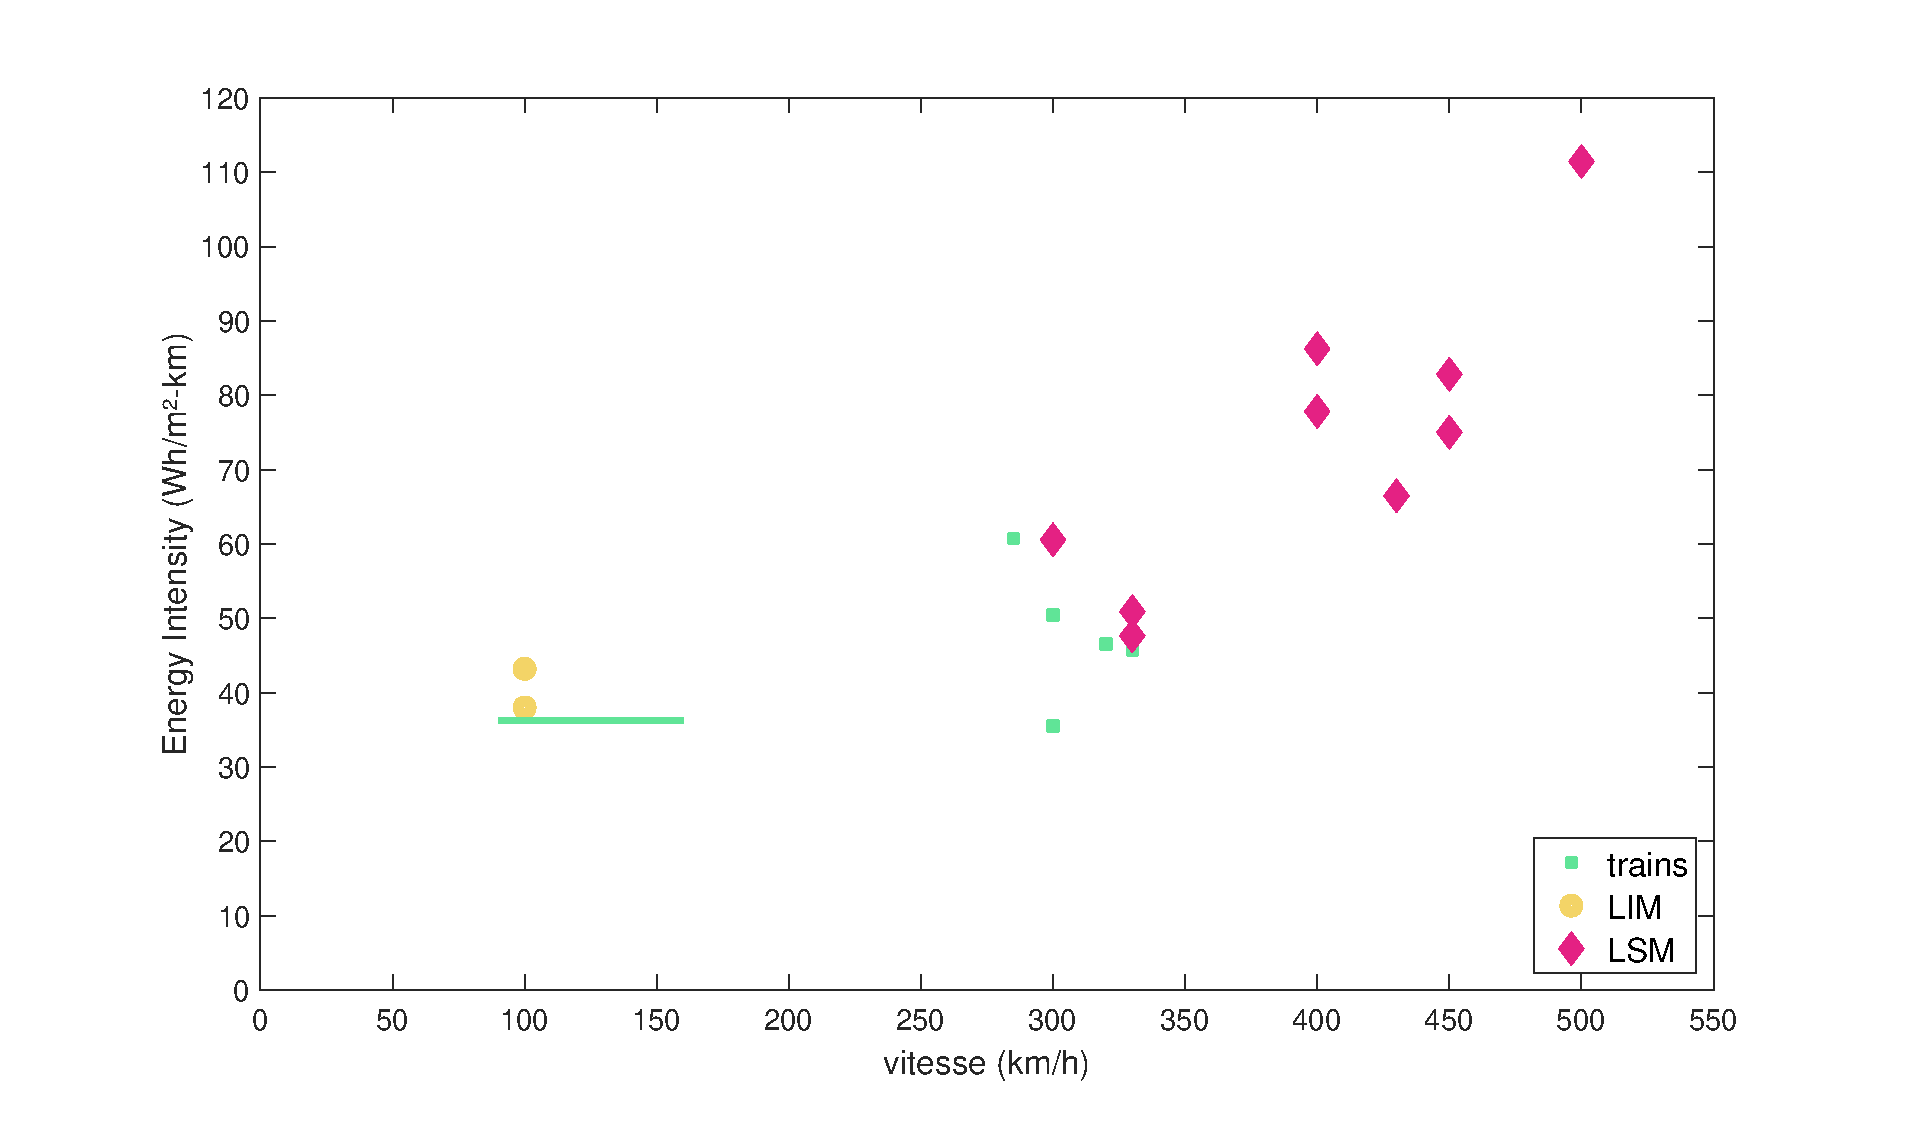
\includegraphics{fig/EI.eps}}
  \label{energy intensity}
  \caption{Intensité énergétique selon les vitesses et les technologies\bettercite{linimo}{ei}{railwayhandbook}}
\end{figure}



\pagebreak %page 14
\tab En comparant les trains et les technologies maglev à une vitesse commerciale de 300-330 km/h, les technologies maglev semblent tout aussi efficaces que les technologies roue-rail, les seules variations pouvant venir des points cités précédemment.
La similarité des résultats obtenus entre les différentes technologies peut s’expliquer en deux points :
\begin{itemize}
  \item Premièrement, en reprenant le PFD appliqué aux trains, on constate qu’à vitesse constante, la seule consommation d’énergie (hors auxiliaires) sert à contrer les forces résistives, qui restent dans le même ordre de grandeur pour les différentes technologies\bettercite{ei},
  \item Deuxièmement, les rendements des chaînes de traction des technologies restent très élevés.
\end{itemize}

\tab En effet, la chaîne de traction des trains est connue pour être très efficace.
Le rendement de celle-ci commençant à 78\% pour les très faibles vitesses et dépassant rapidement 90\% pour les vitesses élevées\bettercite{thesetgv}.
Les maglev équipés de moteurs LSM sont avantagés par le système de sustentation EDS.
Ceux-ci ont un rendement se rapprochant fortement de celui de la chaîne de traction des trains avec des valeurs tournant entre 80\% et 85\% et pouvant monter jusqu’à 92\% en optimisant la longueur des sections de voie\bettercite{coloradomaglev}. \\
\linebreak
\tab En nous intéressant aux très fortes vitesses, on constate une augmentation de l’Intensité Énergétique, ce qui est cohérent car pour les vitesses élevées, les forces résistives augmentent avec le carré de la vitesse.
En prenant ces différents points en considération, l’augmentation de consommation sur les lignes LSM n’est pas alarmante.
La mesure réalisée sur le matériel roulant de la ligne Chuo Shinkansen (MLX-01 ou SCmaglev) à 500km/h peut s’avérer être une surestimation en raison des conditions d’essais, réalisés en tunnels là où les forces résistives sont plus élevées. \\
\linebreak
\tab Pour les faibles vitesses, le constat reste similaire.
Il n’y a pas de grandes différences entre les trains et les maglev à moteurs LIM.
Cependant, les essais sur les lignes LIM  restent faibles et les valeurs indiquées pourraient évoluer avec les recherches futures.
En comparant d’une façon similaire ces deux technologies, nous pourrions penser que l’intensité énergétique des systèmes LIM resterait supérieure à celle des trains pour les mêmes vitesses, le rendement des systèmes LIM étant estimé entre 70\% et 77\%\bettercite{coloradomaglev}.
Il faudrait donc apporter plus d’énergie en entrée pour contrer ces pertes causées par les fuites magnétiques, dues à l’entrefer (écart entre le rail et le véhicule). \\
\linebreak
\tab On peut donc en conclure que la consommation d’énergie lors des trajets n’est pas un facteur décisif quant au choix de la technologie du véhicule guidé.
L’évolution de ce facteur au cours des 50 dernières années ainsi que son évolution potentielle dans les années futures reste faible\bettercite{transportationenergy} ; il ne sera donc toujours pas impactant.



\pagebreak %page 15
\begin{addmargin}[30px]{0px} \subsubsection*{Maintenance}\end{addmargin}

\tab Dans le cas d'un véhicule LIM, l'absence de contact direct entre le véhicule et la voie ainsi que le nombre de pièces mobiles bien plus faible que pour un train entraînent un coût de maintenance inférieur et une durée de vie supérieure.
Pour un véhicule LSM, malgré l'absence de contact direct entre le véhicule et la voie ainsi que le nombre réduit de pièces mobiles, la maintenance entraîne un coût très élevé en raison des technologies extrêmement développées, complexes et coûteuses tout au long de la voie.
De plus, celle-ci subit des efforts électromagnétiques extrêmes à une fréquence très élevée, nécessitant une maintenance accrue. \\
\linebreak
\tab Les coûts de maintenance des véhicules maglev restent cependant supérieurs à ceux d'un train en raison de la faible implémentation de ces lignes et donc du faible nombre de pièces de rechange.
Celles-ci ne sont parfois plus produites et nécessitent donc à nouveau une production, comme par exemple pour le LINIMO. \\
\linebreak
\linebreak
\tab Les coûts nécessaires à la construction des lignes ainsi qu'à leur entretien et à celui des véhicules montrent une forte différence entre le train et les véhicules maglev.
Ainsi, en comparant les lignes LSM aux LGV et les lignes LIM aux lignes de trains conventionnelles, il apparaît que les lignes maglev sont beaucoup plus chères à construire.
Concernant la maintenance des lignes et des véhicules, les maglev sont encore une fois plus chers que les trains.
Cependant, une baisse des coûts de maintenance des lignes et véhicules LIM est envisageable avec leur développement, au contraire des lignes LSM qui demandent une très forte maintenance aux vues des technologies des lignes.
Seule la consommation énergétique varie peu en gardant les mêmes comparaisons.



\pagebreak %page 16
\subsection{Autres critères de choix}
\tab Après avoir constaté les fortes performances des technologies maglev en terme de trajet et leurs forts coûts qui y sont associés, il est aussi important de mentionner certains autres points qui pourraient se révéler critiques lors d'une planification de ligne.

\begin{addmargin}[30px]{0px} \subsubsection*{Rampes}\end{addmargin}
\tab Lors de notre application du PFD réalisée dans la section accélération, nous avons émis des conditions de comparaison telle que la force résistive R$_p$ soit nulle.
Ce terme décrit la déclivité de la voie en rampe ou en pente et s’exprime de la forme : \\
$$R_p = Mgi$$
avec : \\
\begin{itemize}
  \item i l'angle exprimé en mm/m,
  \item M la masse du véhicule complet,
  \item g la constante d’accélération gravitationnelle.
\end{itemize}
\tab L’objectif ici est de pouvoir prendre une rampe maximale (i le plus élevé), sans pour autant avoir une force résistive trop contraignante.
Pour maximiser les rampes appréhendables, il faut encore une fois maximiser l’effort de traction ou minimiser la masse de notre matériel roulant. \\
\linebreak
\tab En reprenant encore une fois les données de la section accélération sur la masse surfacique (de 830 kg/m², 820 kg/m² et 650 kg/m² respectivement pour le TGV, le LIM et le LSM) ainsi que leur longueur (de 200m ou 450m, 80m à 120m et 30m à 50m respectivement pour le TGV, le LIM et le LSM), on trouve que le train est bien plus désavantagé sur la masse déplacée que les deux technologies maglev, de part sa forte masse surfacique et sa longueur.
En regardant les lignes actuellement existantes on trouve les résultats suivants : \\
\begin{itemize}
  \item i$_{train}$ entre 30\textperthousand et 35\textperthousand
  \item i$_{LIM}$ entre 60\textperthousand et 70\textperthousand\bettercite{incheonairport}
  \item i$_{LSM}$ environ 40\textperthousand\bettercite{chuoshinkansen} (Résultat sur la ligne Chuo Shinkansen)
\end{itemize}

\tab Les résultats ci-dessus font sens au vu des puissances mis en jeu\cfannexe{2}.
Cependant il reste important de préciser que les résultats de déclivité pour le train et le LIM sont réalisés en mode dégradé (à vitesse réduite), alors que la ligne shinkansen étant en zones fortement dénivelées, les rampes restent faibles pour préserver une grande vitesse.
En considérant comme pour les autres technologies un mode dégradée, les rampes franchissables pour les lignes LSM seraient de l’ordre de 100 \textperthousand \:à 120 \textperthousand\cfannexe{2}\bettercite{maglevus}.



\pagebreak %page 17
\begin{addmargin}[30px]{0px} \subsubsection*{Rayons de courbures et dévers}\end{addmargin}
\tab Pour des raisons de sécurité, les rayons de courbures sont un point important du tracé en plan d'un train ou d'un véhicule maglev. \\
Dans le cas d’un véhicule LIM, pour une vitesse de 80 km/h, le rayon de courbure moyen varie entre 500 et 800 mètres\bettercite{incheonairportev}{changshadata} \, selon les lignes.
Quant au train, pour cette même vitesse le rayon de courbure moyen n’est que de 350 m\bettercite{thesetgv}.
Concernant les véhicules LSM, pour des vitesses bien plus élevées de 400 km/h et de 500 km/h, celui-ci est respectivement de 4200 et 6500 m\bettercite{rayonLSM}, contre 5500 m pour un train à 350 km/h\bettercite{thesetgv}. \\
\linebreak
Pour des raisons de confort et de sécurité, l’accélération verticale en courbe ne dépasse pas +0.1g et l’accélération transversale ne dépasse pas 0.03g\bettercite{deversLSM}.
Pour diminuer ces valeurs, le rayon de courbure peut être augmenté ou un dévers peut être ajouté.
Pour les mêmes rayons et vitesses que précédemment et en considérant une insuffisance de dévers, on obtient un angle de dévers d’environ 3° pour les maglev LIM\bettercite{changshadata} \, contre 6° pour le train et 15° pour les maglev LSM\bettercite{deversLSM} \, contre environ 7° pour le train.
Les véhicules LIM étant principalement des véhicules urbains, il est nécessaire d’avoir un rayon de courbure plus élevé que pour un train pour des raisons de confort.
Dans le cas des véhicules LSM, le dévers plus élevé permet d’avoir un rayon de courbure plus faible que pour les trains. \\

\begin{addmargin}[30px]{0px} \subsubsection*{Impact des conditions climatiques}\end{addmargin}
\tab Un dernier point à comparer est la capacité des technologies à être opérationnelles indépendamment des conditions climatiques.
Ici le contact roue-rail montre encore sa faiblesse.
Les trains sont connus pour avoir énormément de retard lors de faibles températures, ainsi qu’en automne avec les feuilles tombant sur les voies et limitant encore plus l’adhérence déjà faible de celui-ci. \\
\tab Les technologies maglev suppriment tout contact avec le rail et maintiennent leurs positionnement grâce à un champ électromagnétique.
Le champ électromagnétique n’étant que très légèrement influencé par la présence d’objets non métalliques sur la voie, et les lignes maglev étant généralement surélevées, celles-ci ne sont donc pas impactées par les conditions climatiques.



\pagebreak %page 18
\section*{Conclusion}
\tab Les différents points étudiés nous permettent d’établir les différentes situations où il est préférable d’opter pour des technologies maglev plutôt que pour des technologies ferroviaires classiques.
Grâce aux fortes capacités en pentes des deux technologies maglev, il pourrait être préférable de les choisir pour des zones à forts dénivelés.
De plus, les capacités d’accélération et de décélération accrues des technologies LIM permettraient une diminution des temps de trajets sur des réseaux régionaux où celui-ci est important.
De même sur les grandes lignes avec les technologies LSM, qui en plus d’avoir des capacités d’accélération et de décélération exceptionnelles ont une vitesse commerciale très élevée.
Cependant le coût kilométrique pour la construction de ces lignes reste 3 fois plus élevé que pour les lignes classiques et à grandes vitesses, ce qui limite énormément leur déploiement. \\
\linebreak
\tab Il est aussi important de se rappeler que même si nous avons trouvé des résultats répondant au mieux à notre problématique, ceux-ci peuvent rester imprécis dû à la multitude de programmes de traction ainsi qu’à la faible présence des technologies maglev et au nombre de recherches limitées sur le sujet.
Ce si faible développement peut être expliqué par plusieurs raisons : \\
\begin{itemize}
  \item Premièrement les principaux pays recherchant et développant ces systèmes (Japon, Chine, Allemagne,...) sont des pays avec des réseaux ferroviaires déjà très développés. Ces pays préfèrent maintenir leur réseau déjà existant et dans le cas où ils veulent le développer, ceux-ci préfèrent tout de même rester sur un système ferroviaire classique pour limiter les prises de risques, malgré les potentiels avantages que ce système pourrait apporter dans certains cas\bettercite{maglevus}.
  \item De plus, une raison historique s’ajoute. Les premières traces de recherches sur les technologies maglev remontent en 1908 avec un brevet déposé par Tom.L.JohnSon\bettercite{firstpatent}, avec les premiers tests réalisés dans les années 1940.
\end{itemize}

\begin{figure}[H]
  \label{reseau ferre}
  \centering
  \scalebox{0.48}
  {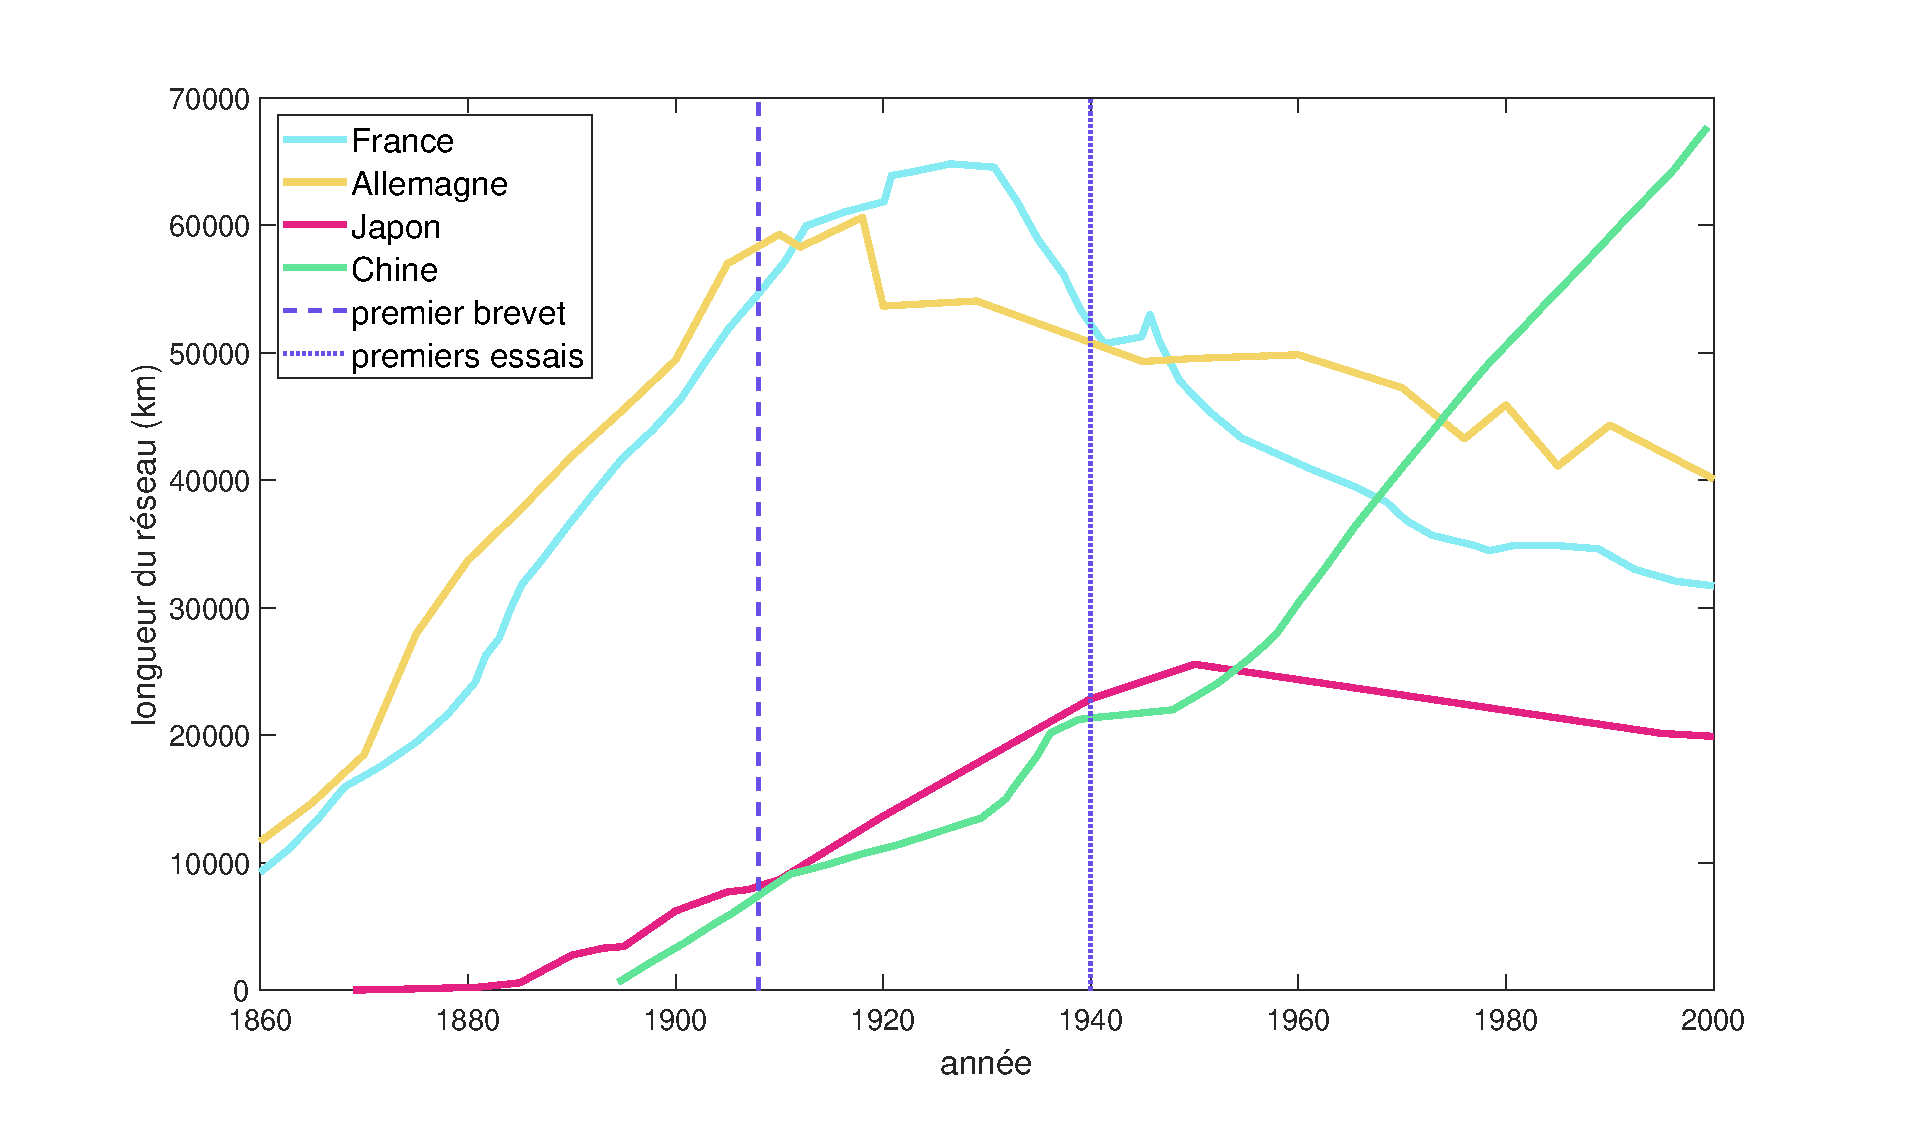
\includegraphics{fig/RF.eps}}
  \caption{Evolution des Réseaux Ferrés selon les années\bettercite{rffrance}{rfallemagne}{rfchine}{rfjapon}}
\end{figure}



\pagebreak %page 19
\begin{addmargin}[30px]{0px}
  Le premier brevet est arrivé en plein essor du développement des différents réseaux ferrés et les premiers essais lors du pic de développement de ceux-ci.
  Les recherches et applications de ces technologies sont arrivées trop tardivement par rapport au développement des différents réseaux ferrés, ce qui explique la situation actuelle quant à celui des technologies maglev. \\
\end{addmargin}



\pagebreak %page 20
\begin{appendix}
  \section{Annexes}
  \subsection{Liste des lignes ouvertes ou en développement}
  \label{annexe 1}

  \bgroup
  \def\arraystretch{1.2}
  \begin{adjustwidth}{-40px}{-40px}
    \begin{tabular}{|c|c|c|c|c|c|c|}
      \hline
      ligne                                                                                & pays         & longueur & vitesse & coût        & sustentation & propulsion \\
      \hline
      Shanghai Transrapid                                                                  & Chine        & 30.5 km  & 430km/h & 1077M\euro  & EDS + EMS    & LSM        \\
      \hline
      Changsha Express\bettercite{changshadata}{changshasources}                           & Chine        & 18.5km   & 120km/h & 607M\euro   & EMS          & LIM        \\
      \hline
      Line S1 Beinjing                                                                     & Chine        & 10km     & 110km/h & ?           & EMS          & LIM        \\
      \hline
      Chengdu Xinzhu                                                                       & Chine        & 4.5km    & 160km/h & 86M\euro    & EMS          & LIM        \\
      \hline
      UTM-02 Daejeon\bettercite{koreamaglevprogram}                                        & Corée du Sud & 1km      & 100km/h & ?           & EMS          & LIM        \\
      \hline
      Incheon Itl Airport\bettercite{koreamaglevprogram}{incheonairport}{incheonairportev} & Corée du Sud & 6.1km    & 80km/h  & 187M\euro   & EMS          & LIM        \\
      \hline
      Nagoya Linimo\bettercite{linimo}                                                     & Japon        & 8.9km    & 100km/h & 466M\euro   & EMS          & LIM        \\
      \hline
      Chuo Shinkansen\bettercite{chuoshinkansen}                                           & Japon        & 285.6km  & 500km/h & 55000M\euro & EDS + roues  & LSM        \\
      \hline
    \end{tabular}
  \end{adjustwidth}
  \egroup



  \pagebreak %page 21
  \subsection{Annexe 2 : Diagrammes effort-vitesse}
  \label{annexe 2}
  \begin{figure}[H]
    \label{effort vitesse train}
    \centering
    \scalebox{0.51}
    {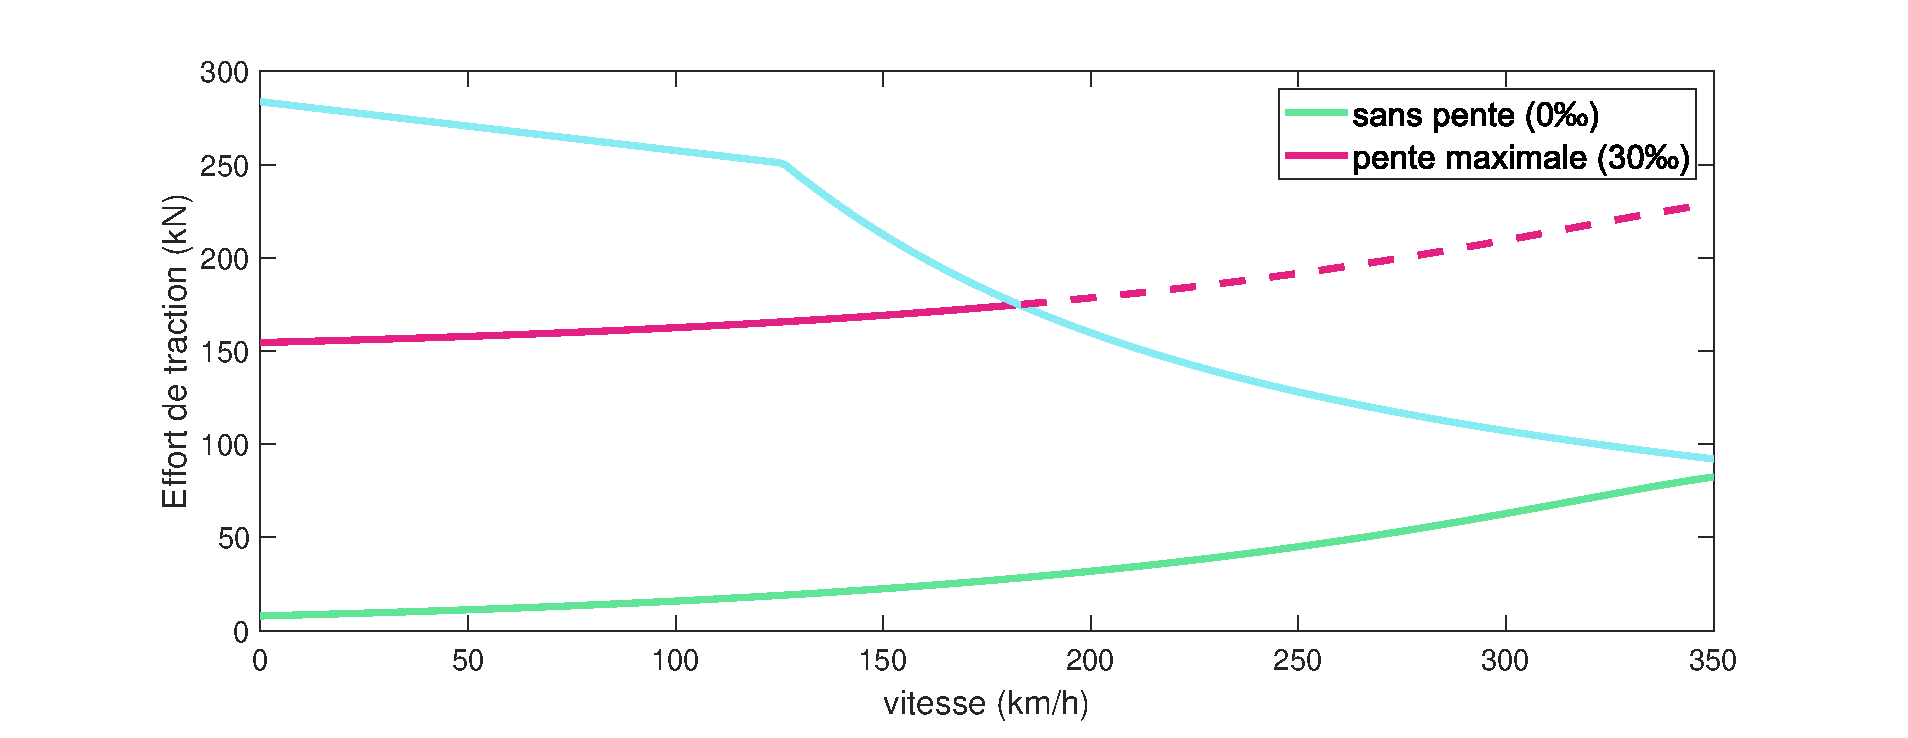
\includegraphics{fig/EVtrain.eps}}
    \caption{Diagramme effort-vitesse du Velaro (automotrice à grande vitesse)\bettercite{maglevus}}
  \end{figure}

  \begin{figure}[H]
    \centering
    \label{effort vitesse LIM}

    \scalebox{0.51}
    {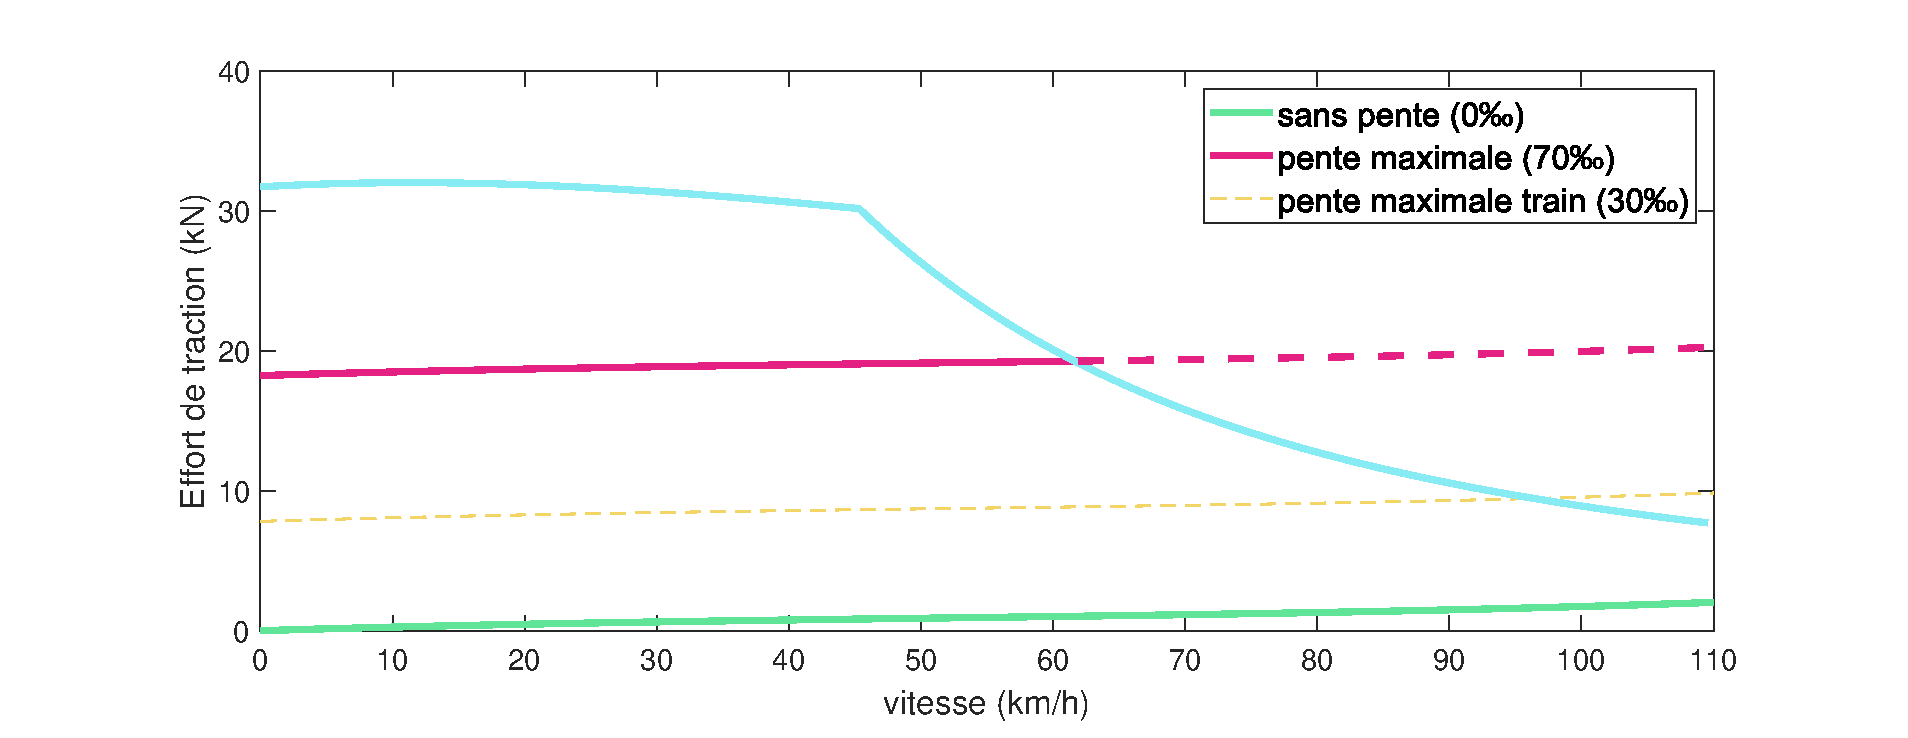
\includegraphics{fig/EVLIM.eps}}
    \caption{Diagramme effort-vitesse de l'ECOBEE (LIM : Incheon International Airport)\bettercite{incheonairportev}}

  \end{figure}
  \begin{figure}[H]
    \centering
    \label{effort vitesse LSM}

    \scalebox{0.51}
    {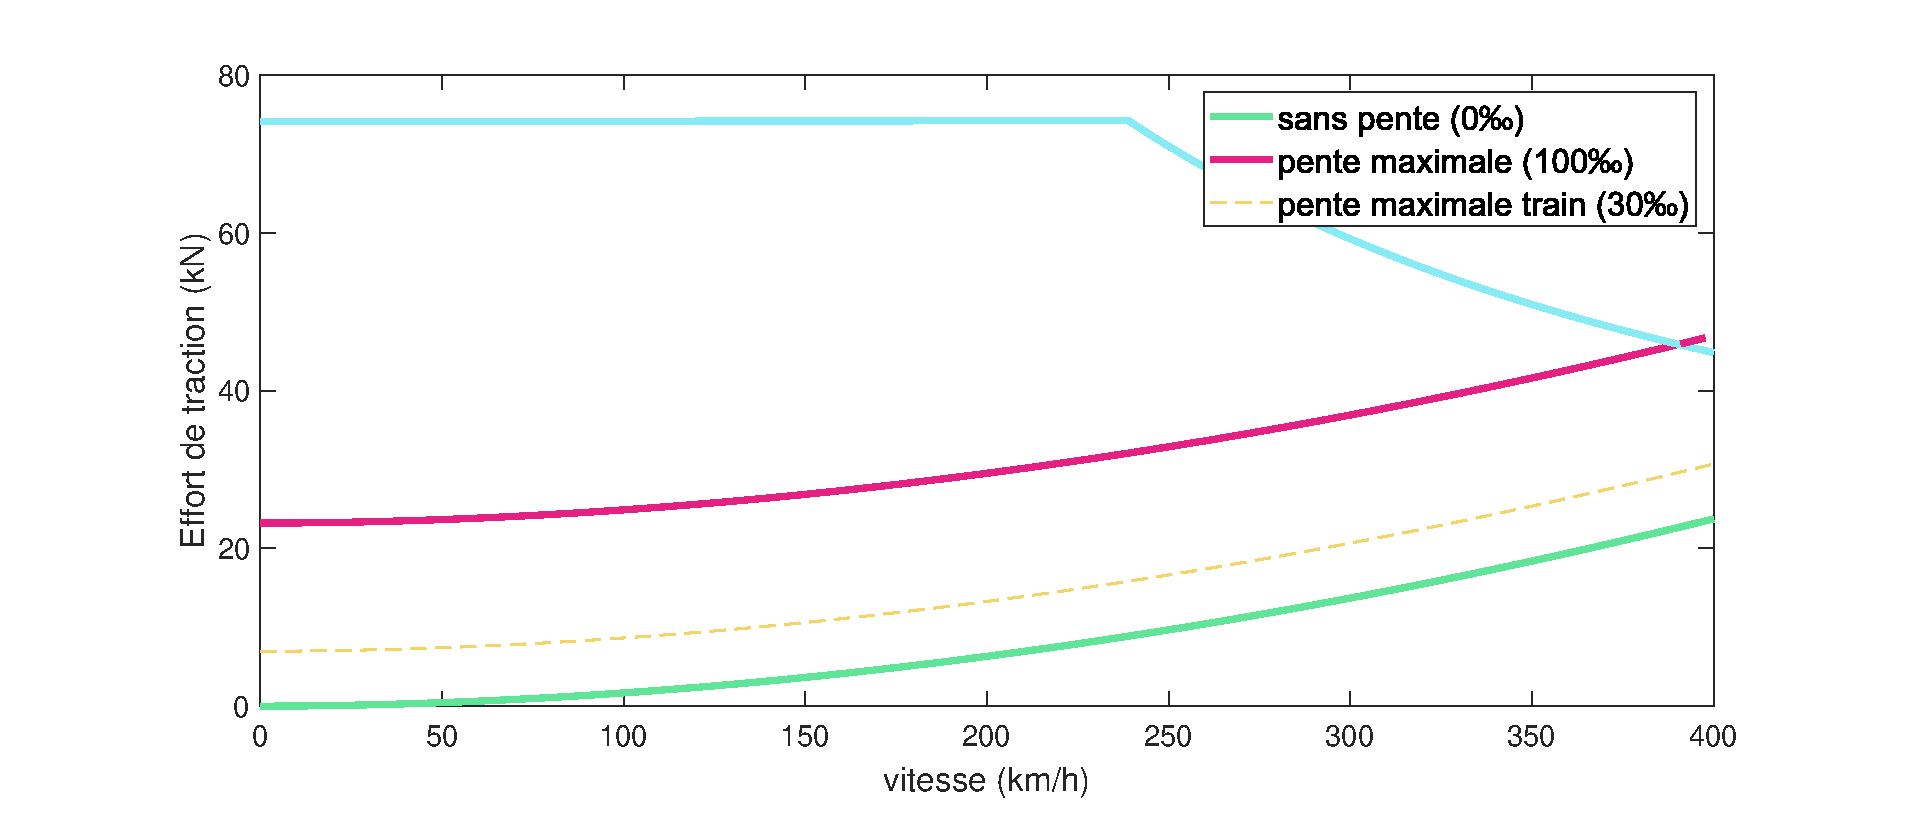
\includegraphics{fig/EVLSM.eps}}
    \caption{Diagramme effort-vitesse du TR-09 (LSM : Shanghai maglev Express)\bettercite{maglevus}}
  \end{figure}



  \pagebreak % page 22
  \subsection{Annexe 3 : Diagrammes vitesse/temps et vitesse/distance}
  \label{annexe 3}

  \begin{figure}[H]
    \centering
    \begin{minipage}[H]{0.49\textwidth}
      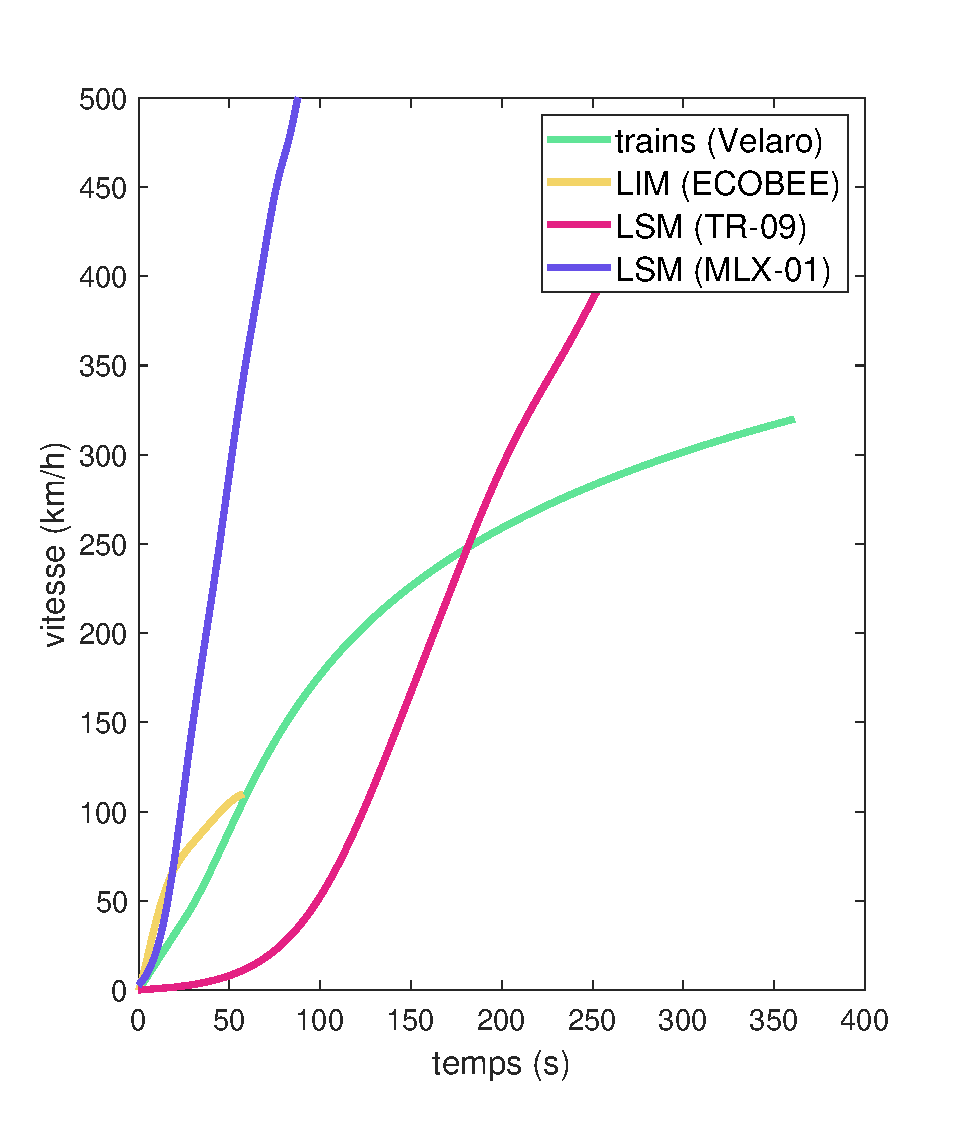
\includegraphics[width=\textwidth]{fig/Atv.eps}
    \end{minipage}
    \hfill
    \begin{minipage}[H]{0.49\textwidth}
      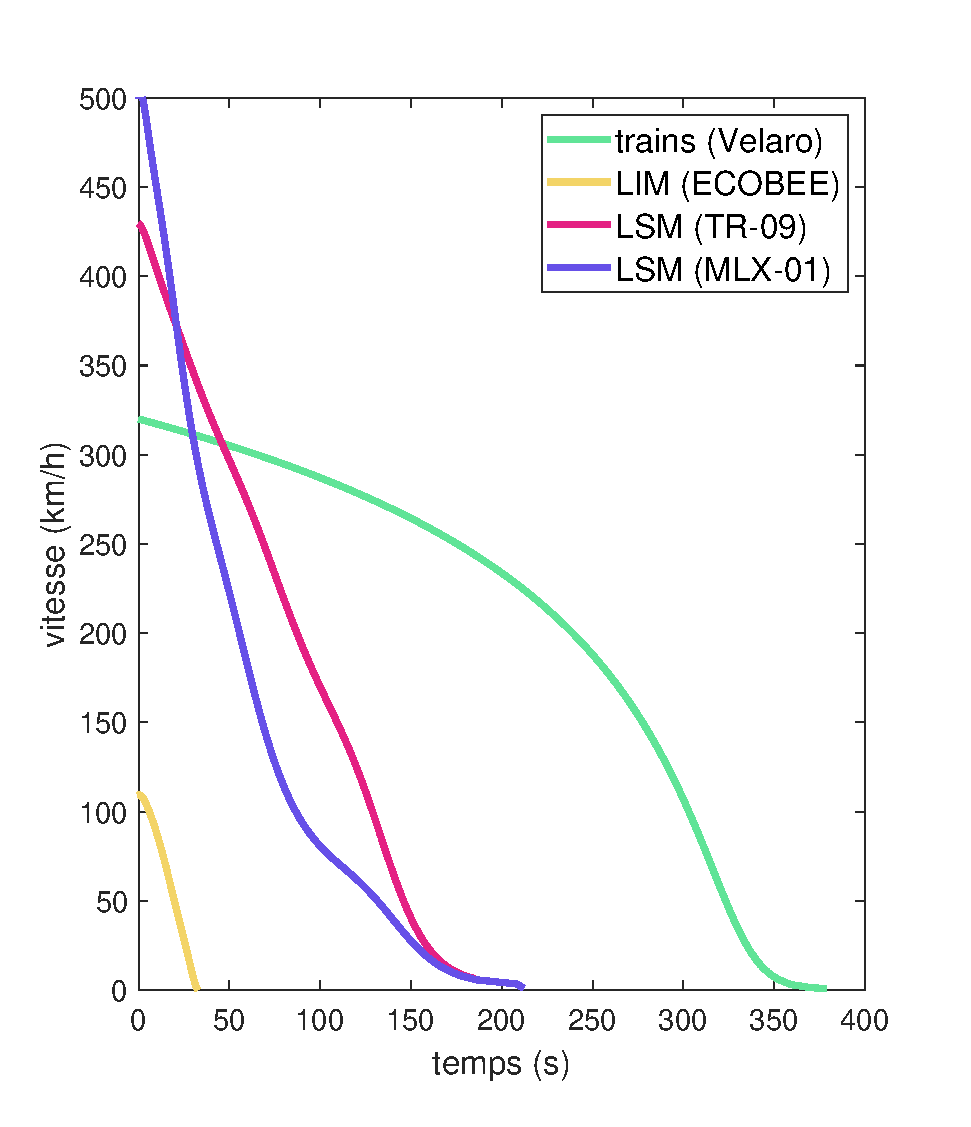
\includegraphics[width=\textwidth]{fig/Dtv.eps}
    \end{minipage}
    \caption{Vitesse selon le temps en accélération et décélération\bettercite{maglevus}{courbeslimlsm}{incheonairportev}}

    \begin{minipage}[H]{0.49\textwidth}
      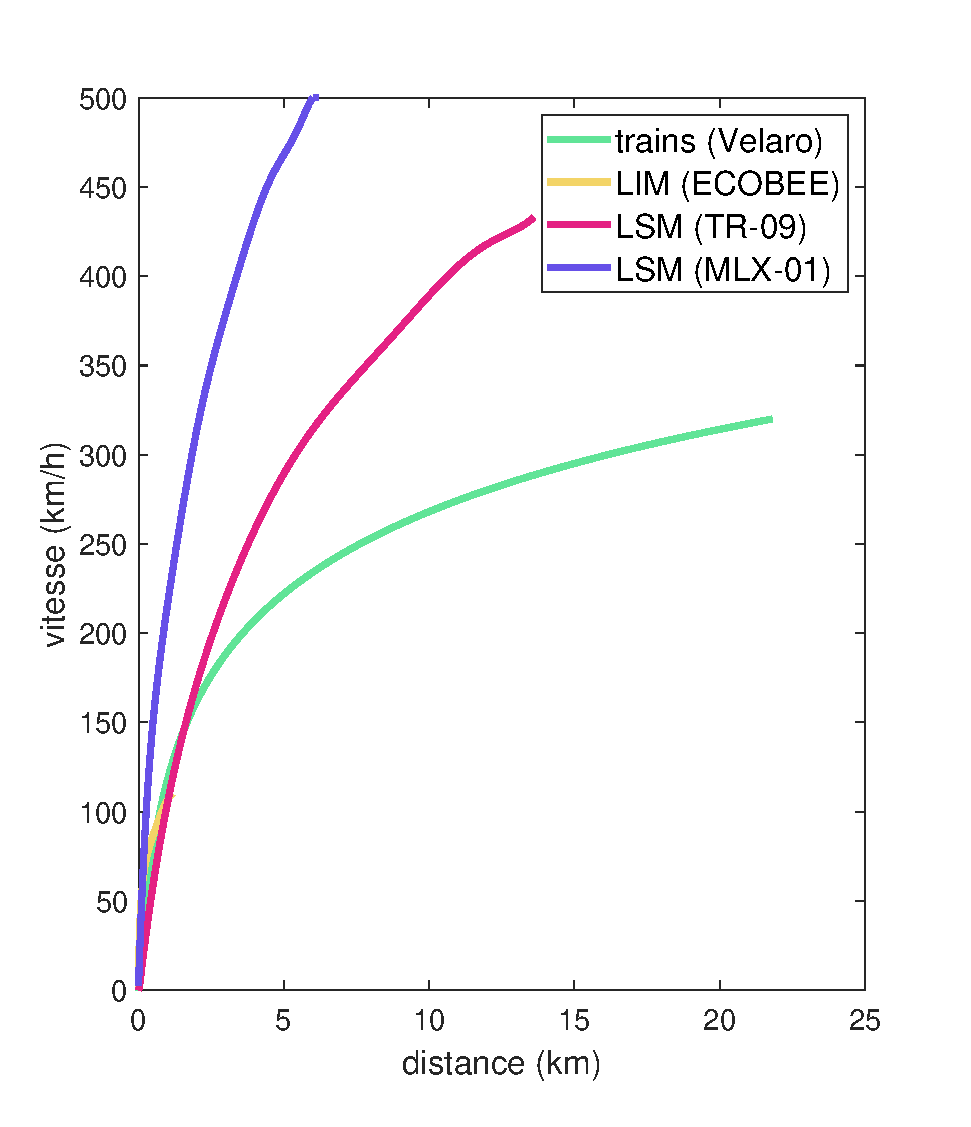
\includegraphics[width=\textwidth]{fig/Adv.eps}
    \end{minipage}
    \hfill
    \begin{minipage}[H]{0.49\textwidth}
      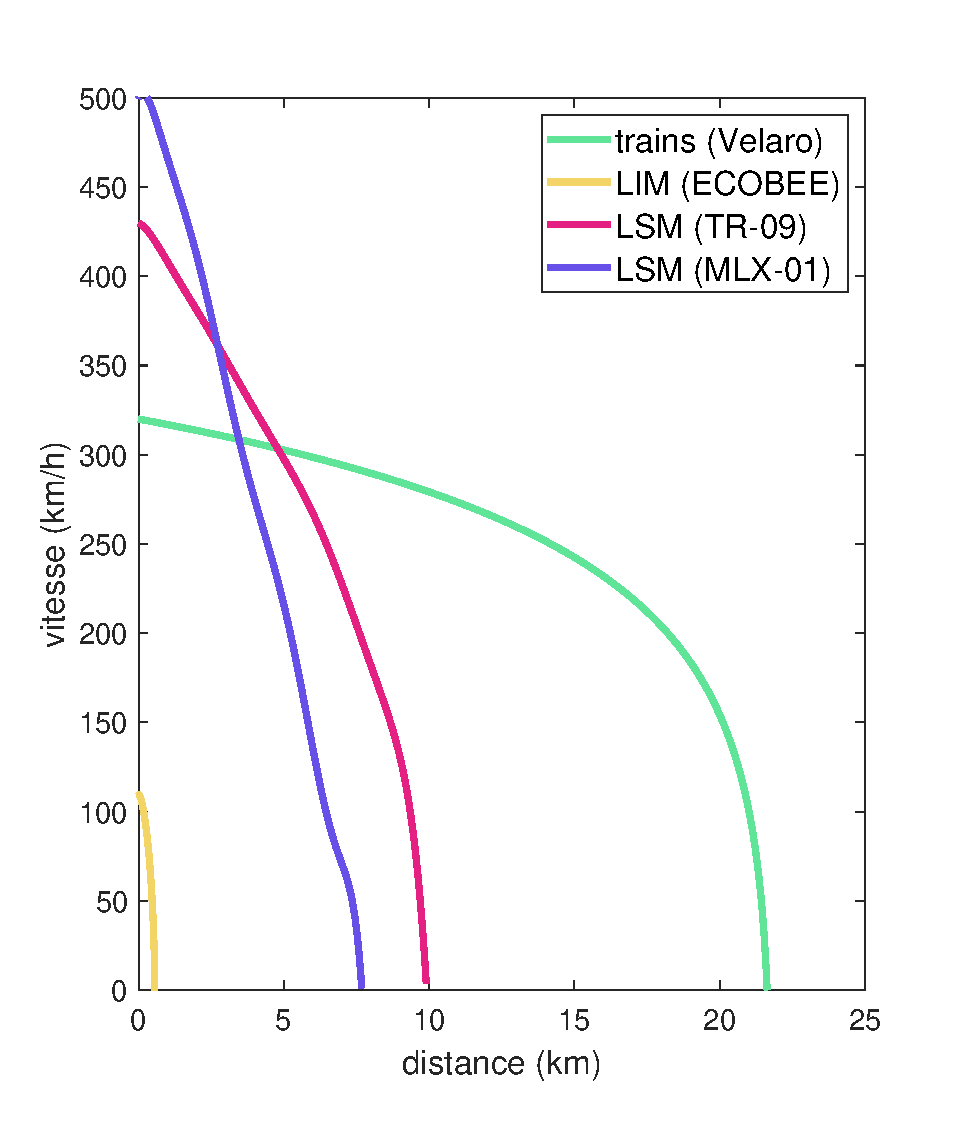
\includegraphics[width=\textwidth]{fig/Ddv.eps}
    \end{minipage}
    \caption{Vitesse selon la distance en accélération et décélération\bettercite{maglevus}{courbeslimlsm}{incheonairportev}}
  \end{figure}

\end{appendix}



\pagebreak %sources
\bibliographystyle{unsrt}
\bibliography{sources.bib}
\nocite{*}
\end{document}